\subsection{Файл с рекордами в игре \q{Block out} и примитивная сериализация}

Многие видеоигры имеют файл с рекордами, иногда называемый \q{Зал славы}.
Древняя игра \q{Block out}\footnote{\url{http://www.bestoldgames.net/eng/old-games/blockout.php}}
(трехмерный тетрис из 1989) не исключение, вот что мы можем увидеть в конце:

\begin{figure}[H]
\centering
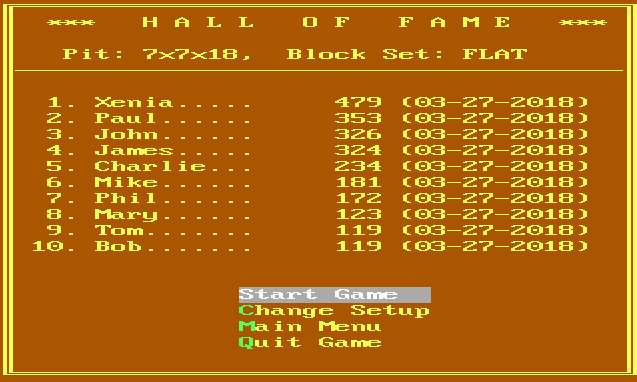
\includegraphics[width=0.7\textwidth]{advanced/550_more_structs/blockout/hs.png}
\caption{Таблица рекордов}
\end{figure}

Мы можем увидеть, что после того как мы всякий раз добаяем свое имя, этот файл меняется: \emph{BLSCORE.DAT}.

\begin{lstlisting}
% xxd -g 1 BLSCORE.DAT

00000000: 0a 00 58 65 6e 69 61 2e 2e 2e 2e 2e 00 df 01 00  ..Xenia.........
00000010: 00 30 33 2d 32 37 2d 32 30 31 38 00 50 61 75 6c  .03-27-2018.Paul
00000020: 2e 2e 2e 2e 2e 2e 00 61 01 00 00 30 33 2d 32 37  .......a...03-27
00000030: 2d 32 30 31 38 00 4a 6f 68 6e 2e 2e 2e 2e 2e 2e  -2018.John......
00000040: 00 46 01 00 00 30 33 2d 32 37 2d 32 30 31 38 00  .F...03-27-2018.
00000050: 4a 61 6d 65 73 2e 2e 2e 2e 2e 00 44 01 00 00 30  James......D...0
00000060: 33 2d 32 37 2d 32 30 31 38 00 43 68 61 72 6c 69  3-27-2018.Charli
00000070: 65 2e 2e 2e 00 ea 00 00 00 30 33 2d 32 37 2d 32  e........03-27-2
00000080: 30 31 38 00 4d 69 6b 65 2e 2e 2e 2e 2e 2e 00 b5  018.Mike........
00000090: 00 00 00 30 33 2d 32 37 2d 32 30 31 38 00 50 68  ...03-27-2018.Ph
000000a0: 69 6c 2e 2e 2e 2e 2e 2e 00 ac 00 00 00 30 33 2d  il...........03-
000000b0: 32 37 2d 32 30 31 38 00 4d 61 72 79 2e 2e 2e 2e  27-2018.Mary....
000000c0: 2e 2e 00 7b 00 00 00 30 33 2d 32 37 2d 32 30 31  ...{...03-27-201
000000d0: 38 00 54 6f 6d 2e 2e 2e 2e 2e 2e 2e 00 77 00 00  8.Tom........w..
000000e0: 00 30 33 2d 32 37 2d 32 30 31 38 00 42 6f 62 2e  .03-27-2018.Bob.
000000f0: 2e 2e 2e 2e 2e 2e 00 77 00 00 00 30 33 2d 32 37  .......w...03-27
00000100: 2d 32 30 31 38 00                                -2018.
\end{lstlisting}

Все записи и так хорошо видны.
Самый первый байт, вероятно, это количество записей.
Второй это 0, и, на самом деле, число записей может быть 16-битным значением, которое простирается на 2 байта.

После имени \q{Xenia} мы видим байты 0xDF и 0x01.
У Xenia 479 очков, и это именно 0x1DF в шестнадцатеричной системе.
Так что значение рекорда, вероятно, 16-битное целочисленное, а может и 32-битное: после каждого по два нулевых байта.

Подумаем теперь о том факте, что и элементы массива, и элементы структуры всегда располагаются в памяти друг к другу впритык.
\myindex{\CStandardLibrary!write()}
\myindex{\CStandardLibrary!fwrite()}
\myindex{\CStandardLibrary!read()}
\myindex{\CStandardLibrary!fread()}
Это позволяет там записывать весь массив/структуру в файл используя простую ф-цию \emph{write()} или \emph{fwrite()}, 
а затем восстанавливать его используя \emph{read()} или \emph{fread()}, настолько всё просто.
Это то, что сейчас называется \emph{сериализацией}.

\subsubsection{Чтение}

Напишем программу на Си для чтения файла рекордов:

\begin{lstlisting}[style=customc]
#include <assert.h>
#include <stdio.h>
#include <stdint.h>
#include <string.h>

struct entry
{
	char name[11]; // включая терминирующий ноль
	uint32_t score;
	char date[11]; // включая терминирующий ноль
} __attribute__ ((aligned (1),packed));

struct highscore_file
{
	uint8_t count;
	uint8_t unknown;
	struct entry entries[10];
} __attribute__ ((aligned (1), packed));

struct highscore_file file;

int main(int argc, char* argv[])
{
	FILE* f=fopen(argv[1], "rb");
	assert (f!=NULL);
	size_t got=fread(&file, 1, sizeof(struct highscore_file), f);
	assert (got==sizeof(struct highscore_file));
	fclose(f);
	for (int i=0; i<file.count; i++)
	{
		printf ("name=%s score=%d date=%s\n",
				file.entries[i].name,
				file.entries[i].score,
				file.entries[i].date);
	};
};
\end{lstlisting}

Нужно добавить атрибут GCC \emph{((aligned (1),packed))}, чтобы все поля структуры были упакованы по 1-байтной границе.

Конечно, это работает:

\begin{lstlisting}
name=Xenia..... score=479 date=03-27-2018
name=Paul...... score=353 date=03-27-2018
name=John...... score=326 date=03-27-2018
name=James..... score=324 date=03-27-2018
name=Charlie... score=234 date=03-27-2018
name=Mike...... score=181 date=03-27-2018
name=Phil...... score=172 date=03-27-2018
name=Mary...... score=123 date=03-27-2018
name=Tom....... score=119 date=03-27-2018
name=Bob....... score=119 date=03-27-2018
\end{lstlisting}

(Нужно добавить, что каждое имя дополнено точками, и на экране, и в файле, вероятно, с эстетическими целями.)

\subsubsection{Запись}

Посмотрим, правы ли мы насчет длины значения очков. Действительно ли там 32 бита?

\begin{lstlisting}[style=customc]
int main(int argc, char* argv[])
{
	FILE* f=fopen(argv[1], "rb");
	assert (f!=NULL);
	size_t got=fread(&file, 1, sizeof(struct highscore_file), f);
	assert (got==sizeof(struct highscore_file));
	fclose(f);

	strcpy (file.entries[1].name, "Mallory...");
	file.entries[1].score=12345678;
	strcpy (file.entries[1].date, "08-12-2016");

	f=fopen(argv[1], "wb");
	assert (f!=NULL);
	got=fwrite(&file, 1, sizeof(struct highscore_file), f);
	assert (got==sizeof(struct highscore_file));
	fclose(f);
};
\end{lstlisting}

Запустим Blockout:

\begin{figure}[H]
\centering
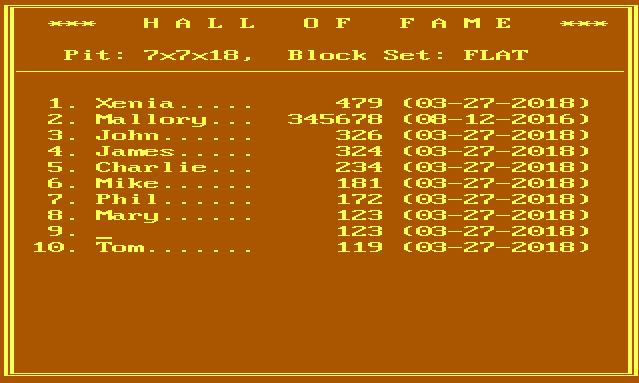
\includegraphics[width=0.7\textwidth]{advanced/550_more_structs/blockout/hs345678.png}
\caption{Таблица рекордов}
\end{figure}

Первые две цифры (1 или 2) пропали: 12345678 стало 345678. Вероятно, это проблемы с форматированием... но число почти корректно.
Заменяю на 999999 и запускаю снова:

\begin{figure}[H]
\centering
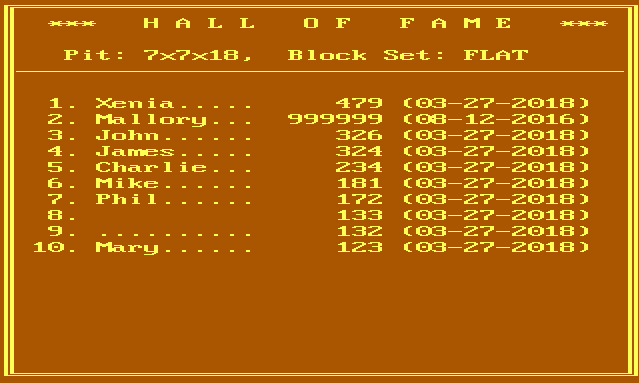
\includegraphics[width=0.7\textwidth]{advanced/550_more_structs/blockout/hs999999.png}
\caption{Таблица рекордов}
\end{figure}

Теперь всё верно. Да, значение очков это 32-битное целочисленное.

\subsubsection{Это сериализация?}

\dots почти.
Сериализация как эта очень популярна в научном и инженерном ПО, где скорость намного важнее чем конвертирование в
\ac{XML} или \ac{JSON} и назад.

Одна очевидная вещь это то что вы, разумеется, не можете сериализировать указатели, потому что каждый раз, когда вы загружаете
файл в память, все структуры могут быть размещены в других местах.

Но: если вы работаете на каком-нибудь маломощном \ac{MCU} с простой \ac{OS} на нем,
и все ваши структуры всегда расположены в тех же местах в памяти, тогда, вы можете сохранять и восстанавливать указатели.

\subsubsection{Случайный шум}

Когда я готовил этот пример, я запускал \q{Block out} много раз и немного играл, чтобы заполнить таблицу рекордов
случайными именами.

И когда было только 3 записи в файле, я увидел это:

\begin{lstlisting}
00000000: 03 00 54 6f 6d 61 73 2e 2e 2e 2e 2e 00 da 2a 00  ..Tomas.......*.
00000010: 00 30 38 2d 31 32 2d 32 30 31 36 00 43 68 61 72  .08-12-2016.Char
00000020: 6c 69 65 2e 2e 2e 00 8b 1e 00 00 30 38 2d 31 32  lie........08-12
00000030: 2d 32 30 31 36 00 4a 6f 68 6e 2e 2e 2e 2e 2e 2e  -2016.John......
00000040: 00 80 00 00 00 30 38 2d 31 32 2d 32 30 31 36 00  .....08-12-2016.
00000050: 00 00 57 c8 a2 01 06 01 ba f9 47 c7 05 00 f8 4f  ..W.......G....O
00000060: 06 01 06 01 a6 32 00 00 00 00 00 00 00 00 00 00  .....2..........
00000070: 00 00 00 00 00 00 00 00 00 00 00 00 00 00 00 00  ................
00000080: 00 00 00 00 00 00 00 00 00 00 00 00 00 00 00 00  ................
00000090: 00 00 00 00 00 00 00 00 00 00 00 00 00 00 00 00  ................
000000a0: 00 00 00 00 00 00 00 00 00 00 93 c6 a2 01 46 72  ..............Fr
000000b0: 8c f9 f6 c5 05 00 f8 4f 00 02 06 01 a6 32 06 01  .......O.....2..
000000c0: 00 00 98 f9 f2 c0 05 00 f8 4f 00 02 a6 32 a2 f9  .........O...2..
000000d0: 80 c1 a6 32 a6 32 f4 4f aa f9 39 c1 a6 32 06 01  ...2.2.O..9..2..
000000e0: b4 f9 2b c5 a6 32 e1 4f c7 c8 a2 01 82 72 c6 f9  ..+..2.O.....r..
000000f0: 30 c0 05 00 00 00 00 00 00 00 a6 32 d4 f9 76 2d  0..........2..v-
00000100: a6 32 00 00 00 00                                .2....
\end{lstlisting}

Первый байт это 3, означая, что здесь 3 записи.
И присутствуют 3 записи.
Но затем мы видим случайный шум во второй части файла.

Шум, вероятно, связан с неинициализированными данными.
Вероятно, \q{Block out} выделил память для 10 записей где-то в \glslink{heap}{куче}, где, очевидно, присутствует
некоторый псевдослучайный шум (оставшийся от чего-то еще).
Затем он выставил первый/второй байт, заполнил 3 записи и затем он никогда не трогал оставшиеся 7 записей,
так что они были записаны в файл как есть.

Когда \q{Block out}, при следующем запуске, загружает файл с рекордами, он читает кол-во записей из первого/второго байта (3)
и полностью игнорирует всё, что идет после.

Это распространенная проблема.
Вернее, не совсем проблема в строгом смысле: ничего не глючит, но лишняя информация может попадать наружу.

\myindex{Microsoft Word}
Microsoft Word версий 90-х часто оставлял куски ранее редактированных текстов в файлах *.doc*.
В те времена это было что-то вроде развлечения, получить \emph{.doc}-файл от кого-то, открыть его в шестнадцатеричном редакторе
и прочитать что-то еще, что редактировалось на том компьютере до этого.

\myindex{Heartbleed}
\myindex{OpenSSL}
Эта проблема может быть куда более серьезная: ошибка Heartbleed\footnote{\url{https://en.wikipedia.org/wiki/Heartbleed}}
в OpenSSL.

\subsubsection{Домашнее задание}

\q{Block out} поддерживает несколько поликубов (flat/basic/extended), размер стакана можно конфигурировать, итд.
И похоже на то, что для каждой конфигурации, \q{Block out} имеет свою таблицу рекордов.
Я заметил, что некоторая информация вероятно сохраняется в файле \emph{BLSCORE.IDX}.
Это может быть домашнее задание для хардкорных фанатов \q{Block out} --- разобраться также и в этой структуре.

Файлы \q{Block out} здесь: \url{http://beginners.re/examples/blockout.zip}
(включая двоичные файлы с рекордами, которые я использовал в этом примере).
Для запуска можно использовать DosBox.

